\section{Domain Analysis}\label{sec:domainAnalysis}
In this section, we specify our blazar observation data and define domain-specific goals and visualization tasks that were identified in consultation with our domain experts. 

\subsection{Blazar Observation Data}\label{sec:BlazarData}
Multiple observatories worldwide collect blazar data; however, their observed properties or units of measurement differ depending on the telescopes being used. 
To reduce uncertainties due to missing observational data and observation errors,
TimeTubesX allows users to fuse multiple datasets for the same blazar from different observatories 
through the automatic handling of potentially different definitions of observed variables~\cite{Fujishiro2018}.
Thus, users can, for example, include data from Hiroshima University and the University of Arizona in the same visualization session. 
TimeTubesX is designed to primarily process datasets acquired by Hiroshima Astrophysical Science Center at Hiroshima University,
which uses a $1.5\mathrm{m}$ Kanata telescope. 

% Observation datasets
The photometric and polarimetric datasets of Hiroshima University include six time-dependent variables: $q$, $u$, $\epsilon_q$, and $\epsilon_u$ for the observed polarization of the light (Fig.~\ref{fig:blazar} (A)), $I$ for the observed intensity (Fig.~\ref{fig:blazar} (B)), and $C$ for the observed color (Fig.~\ref{fig:blazar} (C)).
Linear polarization is represented by $Q$ and $U$, the so-called \textit{Stokes} parameters.
We mainly use fractional values of $Q$ and $U$ where $q = Q / I$ and $u = U / I$, 
because $q$ and $u$ describe the behaviors of a blazar more effectively than $Q$ and $U$~\cite{Uemura2016}.
We call the plane composed of $q$ and $u$ the \textit{Stokes plane}.
$\epsilon_q$ and $\epsilon_u$ act as the observation errors of $q$ and $u$, respectively.
The polarization degree ($PD$) and polarization angle ($PA$) derived from $q$ and $u$ are used to describe the optical polarization.
$PD$ denotes a distance from the origin of the Stokes plane, 
while $PA$ denotes one half of the polar angle in the Stoke plane, as illustrated in Fig.~\ref{fig:blazar}~(A).

The observation frequency differs depending on observatories.
The median observation interval of Hiroshima University is once every two days.
Note that the datasets have missing data due to the rotation and/or revolution of the Earth, bad atmospheric conditions, and so on.
In this paper, we process datasets from Hiroshima University for two blazars: \emph{BL Lac} and \emph{3C 454.3}. 
The two datasets for \emph{BL Lac} contain 285 data samples in each dataset from May 2008 to December 2011, while the one for \emph{3C 454.3} contains 355 data samples from July 2008 to July 2014.

\begin{figure}[tb]
    \centering
        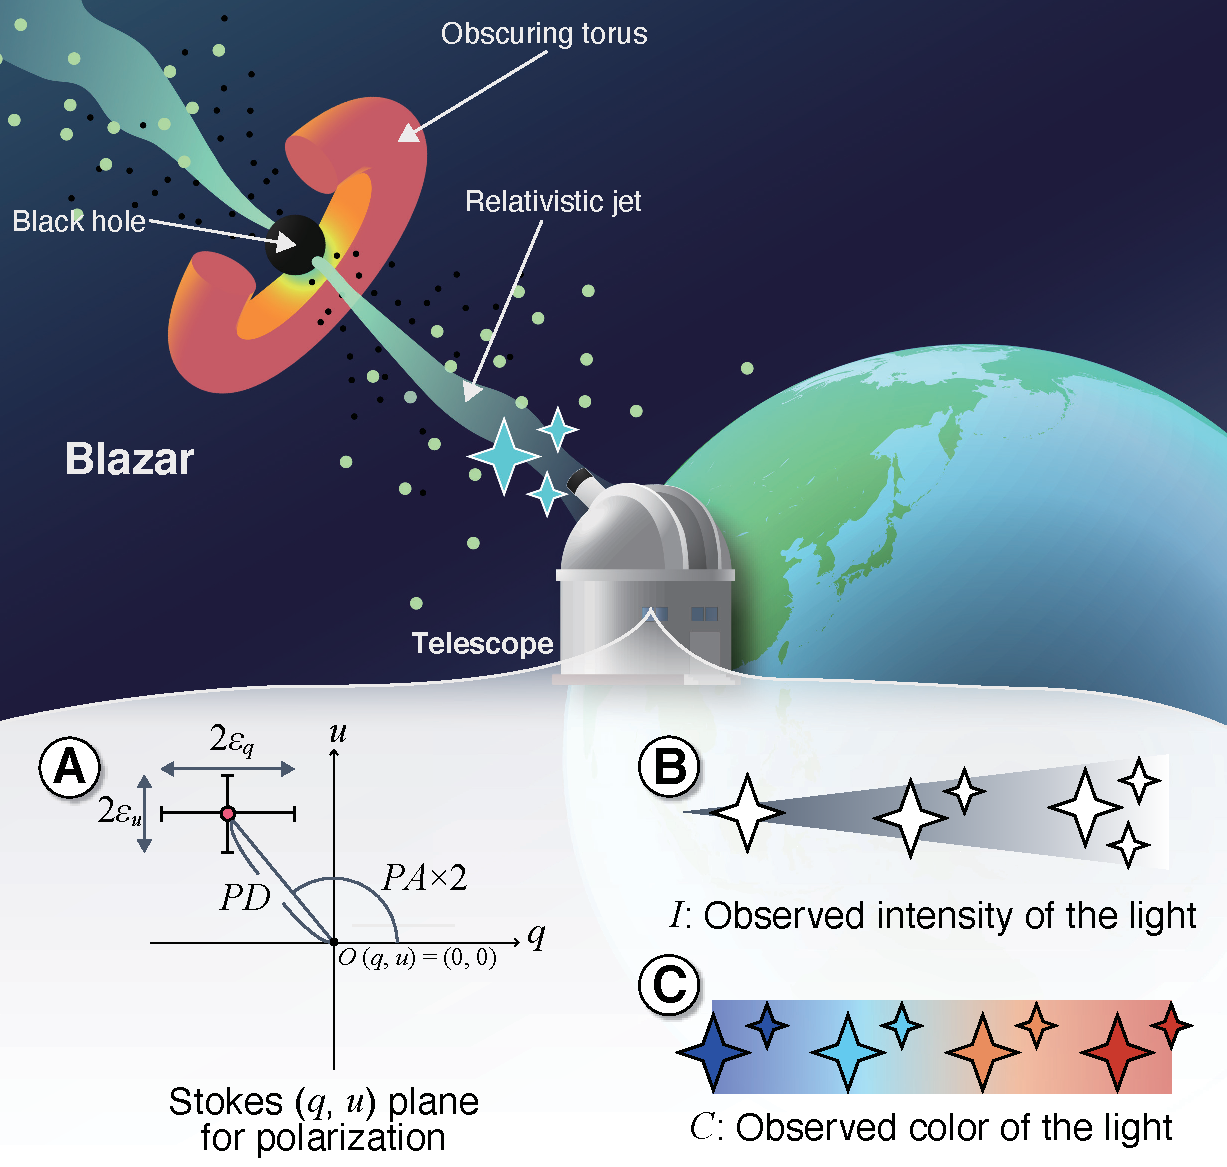
\includegraphics[width=.99\linewidth]{figures/blazar_final.pdf}
    \caption{An observed blazar and its features. A blazar's central black hole emits a relativistic jet toward the Earth.
        The telescope observes its light in terms of (A) polarization, (B) intensity, and (C) color.}
    \label{fig:blazar}
\end{figure}

\subsection{Goals and Visualization Tasks}\label{sec:domainGoalsandTasks}
We interviewed two astronomers at Hiroshima University, one at Stanford University, and four at Boston University to clarify the domain goals and visualization tasks.
The main objective of these astronomers is 
to quickly extract and analyze features in temporal variations of the observed polarization, intensity, and color that are occurring at multiple time intervals. 
TimeTubesX effectively supports the following four domain goals:

\noindent\textbf{G1--Enhance the reliability of blazar observations}. 
Datasets always contain missing data and observation errors. 
Astronomers need to assess whether what they have found is plausible by analyzing the length of missing data periods and the size of errors.

\noindent\textbf{G2--Identify flares and rotations}. 
Astronomers typically pay attention to time intervals with dynamic time variations,
such as flares and rotations.
The analysis of time intervals with such dynamic variations helps astronomers demystify jets' structures.

\noindent\textbf{G3--Locate recurring blazar behaviors}.
Besides well-known behaviors such as flares and rotations, 
recurring patterns or common features can also exist.
Thus, upon finding an interesting pattern or feature, 
astronomers want to locate other time intervals similar to it.

\noindent\textbf{G4--Explore time intervals validating a hypothesis of blazar behaviors}.
Through their analyses or experiences, astronomers sometimes make a hypothesis (e.g., that the flares of a blazar tend to co-occur with a specific polarization variation pattern). 
Astronomers need to address time intervals that might validate the hypothesis.

To attain these four goals, we have identified five visualization tasks that TimeTubesX should support:

\noindent\textbf{T1--Uncertainty-aware visualization.} 
Users should be able to perceive the reliability of data through visualizations. 

\noindent\textbf{T2--Analysis across datasets.} 
To compensate for missing data, 
the system must allow users to aggregate datasets for the same target from different sources.
Analyses across datasets should also be supported to address features that are common to multiple targets.

\noindent\textbf{T3--Analysis of dynamic variations.} 
Time intervals with drastic changes in a short time period and those with unusually large time variations should be automatically extracted.

\noindent\textbf{T4--Similarity analysis of a specific region/shape of interest and time intervals.} 
Users should be able to identify regions/shapes of interest (\emph{ROI}s/\emph{SOI}s) and search for similar time variation patterns at other time intervals without using complex query languages or parameter settings.

\noindent\textbf{T5--Fuzzy search for time intervals similar to a specific ROI/SOI.}
The system should provide not only exact matches between a ROI/SOI and time intervals but also fuzzy or approximate matches. 

To support \textbf{G1}, our previous work, TimeTubes~\cite{Fujishiro2018}, has already supported \textbf{T1} and \textbf{T2}.
Observation errors are encoded in the appearance of the 3D volumetric tube (\textbf{T1}).
An ellipsoidal snapshot and a white cruciform axis appear at each observation timestamp to distinguish missing data (\textbf{T1}).
Analysis across datasets (\textbf{T2}) is supported by visual data fusion, which allows users not only to aggregate multiple datasets for the same blazar but also to effectively compare multiple datasets for the same or a different blazar in a single visualization session.
In this paper, we mainly focus on feature and pattern detection methods to support the remaining three tasks (\textbf{T3}, \textbf{T4}, \textbf{T5}).
Consequently, we have designed an integrated visual analytics framework for blazar observations that supports all identified goals (\textbf{G1}--\textbf{G4}) and tasks (\textbf{T1}--\textbf{T5}).
